\chapter{評価}
複数タスクにかかる所要時間に対し被験者の予測とADLoggerの予測の差異を比較した上で,
ADLogger導入によって,行動・意識の変容が生じるかどうか評価する.
本章ではまず評価概要を説明し,実験結果を示す.最後に,評価実験から得られた結果をもとに考察を行う.

\section{評価実験の概要}
本研究における評価実験の概要を述べる.はじめに,評価実験を行う目的を説明する.
ついで,評価実験を行う手順について説明する.

\subsection{評価の目的}
本研究では,複数タスクにかかる所要時間の予測に関して被験者の予測とADLoggerの予測の差異を比較する事,
ADLogger導入によって,時間管理に対する苦手意識・行動への変化が起こる事を目的としている.

\subsection{実験評価手法}
今回の評価実験では,被験者に時間の長さを教示し,その長さを産生させる時間産生法\cite{Oguro1961}\cite{Tayama2018}を慶應義塾大学の学生男女20名に対し平日と休日(またはそれに準ずる日)にそれぞれ3回(合計6回)に渡って実施した.
始めに,被験者は事前に各自保持しているiPhoneにADLoggerをインストールして貰う.

被験日はまず行動前に朝実施する日常生活動に関して行動名,行動毎の必要時間予測,タスクを連続で行った時の総合必要時間予測を平日と休日(またはそれに準ずる日)に分け申告してもらう.尚,6回の計測を通じて予測を適宜修正できるものとする.
その後,web会議ツールであるzoom\cite{zoom}およびADLoggerを用いながら実際に行動して貰い実測値を計測する.
zoomにおいては全ての行動の開始時/終了時に連絡を行い,実験者が総合時間を計測する.
更に被験者はADLoggerを用いて行動毎の時間を計測する.
4回目の計測日においてはADLoggerのADLogおよびタイマーのカウントアップ表示を閲覧できる状態にしながら計測して貰する.
最終日にはプリケーションによる定性的効果やアプリケーションの改善点を知る為にインタビューを行う.インタビューにて質問する項目は付録Aにて記載した.

評価は上記の全3回における実測値およびアンケートで申告した見積もりとのずれに関して反復測定分散分析(Repeated Measured ANOVA)を行った.

尚,実験期間中(2週間を目安とする)はアプリケーションの予測精度を向上させる点及びアプリケーション使用頻度を分析する為,被験者は実験用に登録した動作を行う度に任意でアプリケーションに計測して貰う様促した.

\section{評価結果}
〜〜ここからは仮置き〜〜\\
本節では,本システムの導入後時間管理に対し与える影響について,本評価実験で得られた評価結果を示す.
まず,3回の計測における見積もりと実測値のずれはの分布は以下の様になった.(図~\ref{fig:hakohige}参照)

\begin{figure}[hb]
	\begin{center}
	\fbox{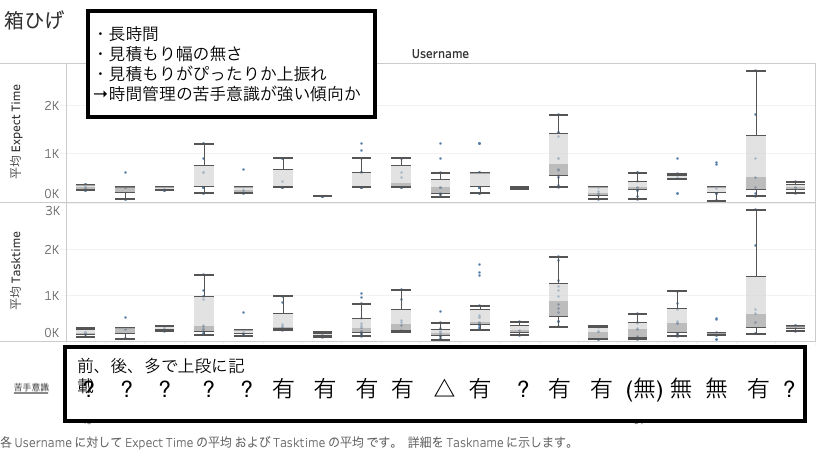
\includegraphics[width=10cm]{images/7/1.png}}
	\caption{3回の計測における見積もりと実測値のずれ(ダミー)}
	\label{fig:hakohige}
	\end{center}
\end{figure}

その上で総合時間及び一日あたりの平均のずれの時間を反復測定分散分析(Repeated Measured ANOVA)を用いて分析したところ,〇〇だった.

また,1回目の計測の総合計時間のずれ(\%)の結果を元に被験者グループを下記の4つに分類した.(実験結果の四分位数を元に調整)

\begin{table}[htb]
  \begin{center}
  \begin{tabular}{|c|c|c|} \hline
    1 & 大前倒し群 & 予測の方がX分以上長かった群  \\ \hline
    2 & 小前倒し群 & 予測の方がX分未満長かった群  \\ \hline
    3 & 小遅延群 & 実測の方がX分以上長かった群  \\ \hline
    4 & 大遅延群 & 実測の方がX分未満長かった群  \\ \hline 
  \end{tabular}
    \caption{バッファモードの選択分岐}
    \label{tb:buffer}
  \end{center}
\end{table}

その後計測2回分の経過をグループ別に表すとそれぞれ図~\ref{fig:2},~\ref{fig:3},~\ref{fig:4},~\ref{fig:5}の様になった.
(※今後オン/オフの評価や各タスクの見積もり推移も評価する可能性があります.)

\begin{figure}[htb]
\begin{center}
\begin{tabular}{c}

  \begin{minipage}[htb]{\linewidth}
  \begin{center}
  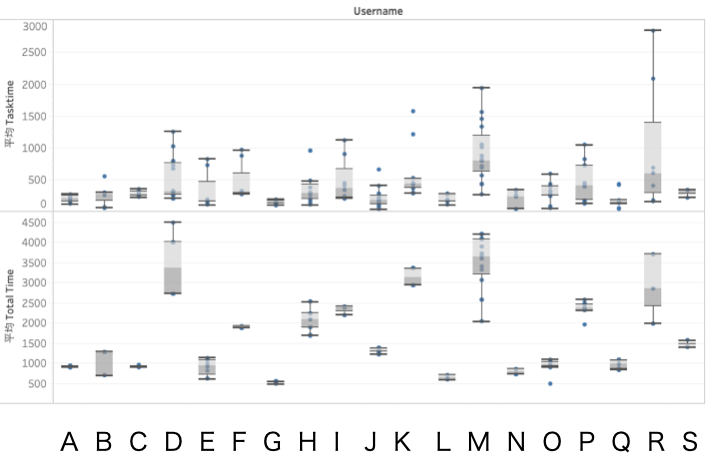
\includegraphics[width=12cm]{images/7/2.png}
  \caption{大前倒し群の推移}
  \label{fig:2}
  \end{center}
  \end{minipage}
  
  \\
  
  \begin{minipage}[htb]{\linewidth}
  \begin{center}
  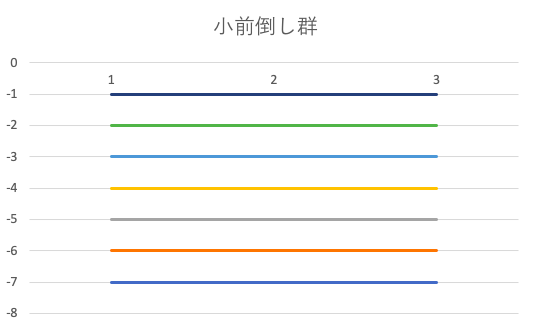
\includegraphics[width=12cm]{images/7/3.png}
  \caption{小前倒し群の推移}
  \label{fig:3}
  \end{center}
  \end{minipage}

\end{tabular}
\end{center}
\end{figure}

\begin{figure}[htb]
\begin{center}
\begin{tabular}{c}

  \begin{minipage}[htb]{\linewidth}
  \begin{center}
  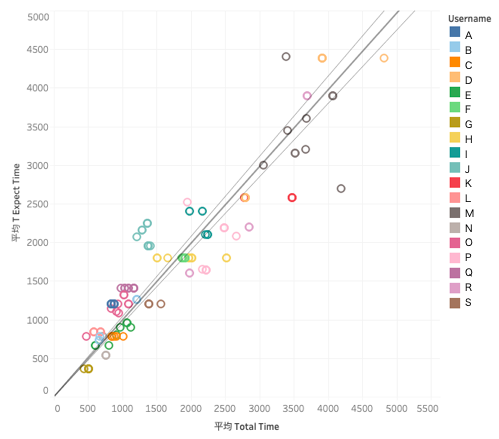
\includegraphics[width=12cm]{images/7/4.png}
  \caption{小遅延群の推移}
  \label{fig:4}
  \end{center}
  \end{minipage}
  
  \\
  
  \begin{minipage}[htb]{\linewidth}
  \begin{center}
  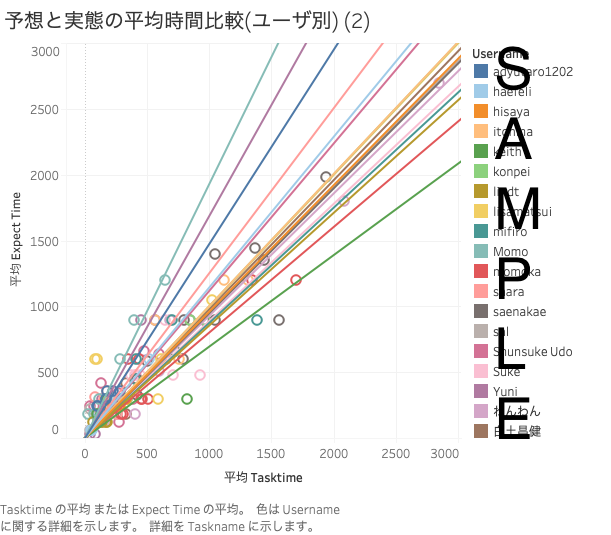
\includegraphics[width=12cm]{images/7/5.png}
  \caption{大遅延群の遷移}
  \label{fig:5}
  \end{center}
  \end{minipage}

\end{tabular}
\end{center}
\end{figure}

\subsection{実験終了後アンケート}
〇〇の様な意見が出された等を書いていく.
\section{考察}
(※詳細は実験データを元に書いていきたいと考えております.一先ず現在考えられるLimitationのみ完結に述べます.)
本実験はデータ数・被験者数が少ない事,短期間である事,一人一人のタスク行動が同一ではない事,時間の見積もり自体は個人間でも均一になりにくい事からデータの偏りが考えられる為更なる収集が必要である.
また,ずれの評価に関しては見積もりの失敗だけでなく複合的な原因が存在する可能性がある為,今後は本評価手法に限定せずに更なる評価実験が必要になると考えられる.
アンケートにおいてはインタビューによる可能性の示唆を元に今後アンケートなどより統計的に評価する意義があると考える.

\section{まとめ}
本章では,評価実験にの概要及び手法についてまとめたた上で,結果・考察を述べた.
次章では,本研究における今後の展望と本論文のまとめを述べる.
